\documentclass{beamer}
\usepackage[utf8]{inputenc}
\usepackage{graphicx}
\usepackage{color}

\usetheme{Warsaw}

\title{TeXloud}
\author{Adrien Bruyère,\\David Ducatel, Meva Rakotondratsima,\\Sidina Biha, Zakaria Bouchakor}
\institute{Université du Havre}
\date{24 Février 2011}

%numerotation des slides
\addtobeamertemplate{footline}{\hfill\insertframenumber/\inserttotalframenumber\hspace{2em}\null}

%changement des couleur
\definecolor{fondtitre}{rgb}{0.20,0.43,0.09}  % vert fonce
\definecolor{background}{rgb}{0.20,0.43,0.09} 

\setbeamercolor{subsection in head/foot}{fg=white, bg=black}
\setbeamercolor{section in head/foot}{fg=black, bg=background!75!black}

\setbeamercolor{structure}{fg=black, bg=fondtitre!40}
%%%%%%%%%%%%%%%%%%%%%%%%%%%%%%fin du préambule%%%%%%%%%%%%%%%%%%%%%%%%%%%%%%%%%%%%%%%%%%%%%%%%%%%%%%%%%%%%%%

\begin{document}

\begin{frame} %%%page de presentation
  \titlepage
\end{frame}


\AtBeginSection[] %%ici pour le plan
{
  \begin{frame}<beamer>
    \frametitle{Plan}
    \tableofcontents[currentsection]
  \end{frame}
}

\section{Introduction}
\subsection{\LaTeX}
\begin{frame}{Introduction -- \LaTeX}
	\begin{itemize}
	\item Langage de description de document.
	\item Publications scientifiques.
	\item Excellent rendu des équations et formules.
	\item Convertible en PDF, PostScript, DVI, HTML , etc.
	\end{itemize}
\end{frame}


\subsection{Projet}
\begin{frame}{Introduction -- Projet}
	\begin{itemize}
	 \item Création de documents \LaTeX.
     \item Plateformes dépourvues de distribution \LaTeX.
     \item Espace de stockage privé.
	\end{itemize}
\end{frame}

\subsection{Environnement}
\begin{frame}{Introduction -- Environnement}
	\begin{block}{Environnement}
		\begin{itemize}
		\item Python
		\item PHP5
		\item JQuery
		\item Mysql
		\item Android
		\item Etc.
		\end{itemize}
	\end{block}
\end{frame}

\subsection{Architecture général}
\begin{frame}{Introduction -- Architecture général}
	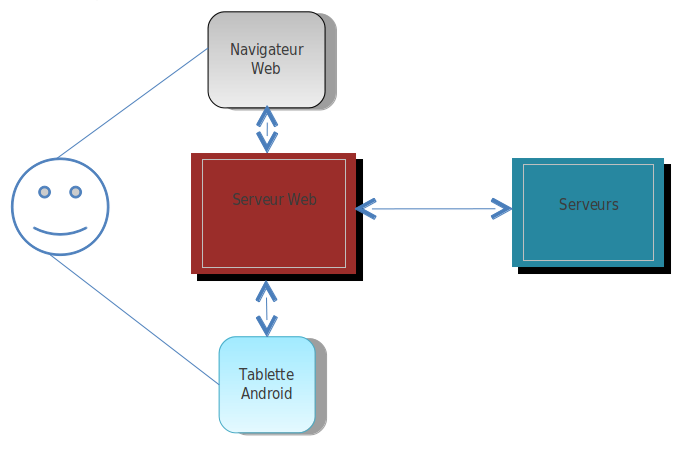
\includegraphics[width=\textwidth]{./images/diaBiha.png}
\end{frame}

\end{document}
